\section{Auswertung}
\subsection{Ersatzschaltbild Transformator}
\begin{enumerate}[label=\alph*)]
	\item Zeichnen Sie das vollständige einphasige Ersatzschaltbild (Sternschaltung) des
	      Transformators.
	      \begin{figure}[h!]
		      \begin{center}
			      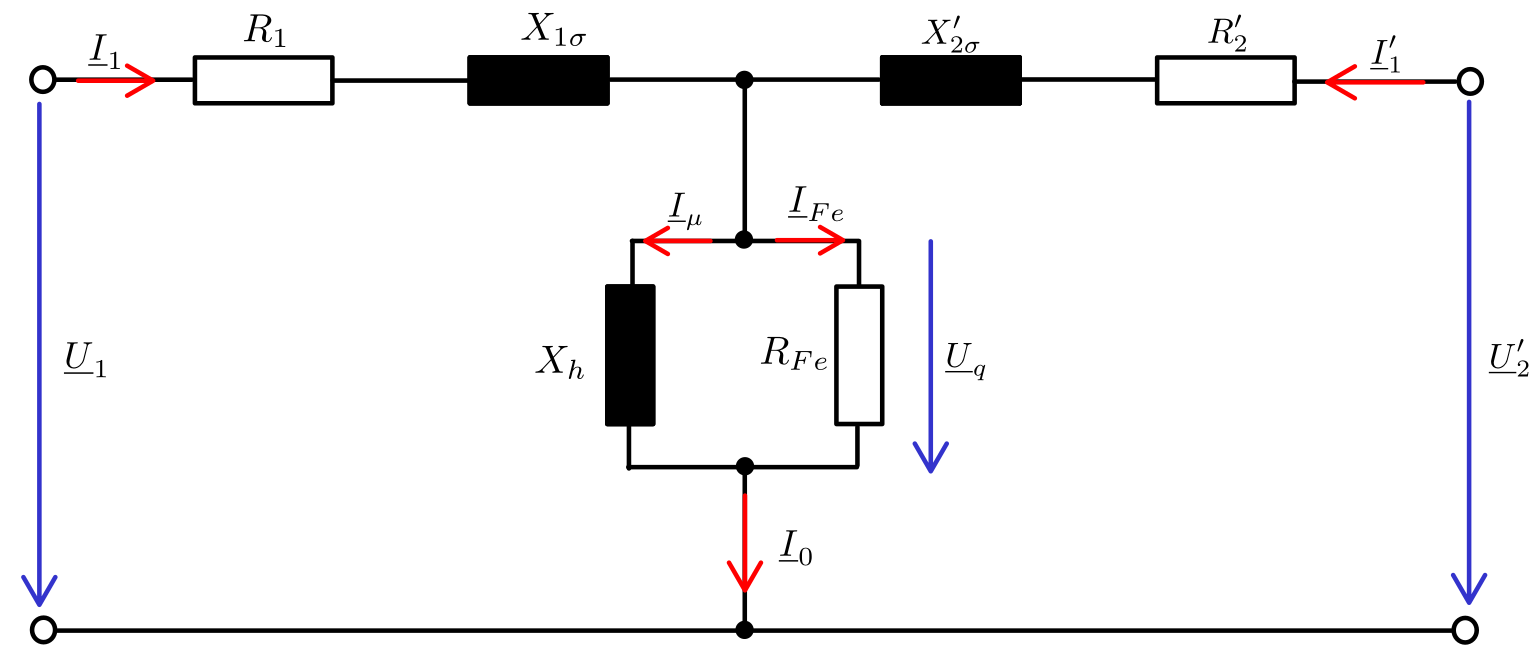
\includegraphics[width=0.95\textwidth]{img/4.1.1.1}
		      \end{center}
		      \caption{}\label{img:4.1.1.1}
	      \end{figure}

	\item Bestimmen Sie die Leistung im Leerlauf auf der Primärseite nach Gleichung (16).
	      \begin{align*}
		      \underline S & = \underline U_{12} \cdot \underline I_1^* + \underline U_{23}\cdot \underline I_3^*                                                 \\
		      \underline S & = 395\ V \cdot e^{j0^\circ} \cdot 0.45\ A \cdot e^{-(-j120^\circ)} + 391\ V \cdot e^{j120^\circ}\cdot 0.45\ A \cdot e^{-(j45^\circ)} \\
		      \underline S & = 326\ VA\cdot e^{j97.6^\circ}
	      \end{align*}

	\item Bestimmen Sie die Wirkleistung im Kurzschlussfall auf der Sekundärseite nach
	      Gleichung (16). Gehen Sie dabei von einem symmetrischen System aus.
	      \begin{align*}
		      \underline S & = \underline U_{12} \cdot \underline I_1^* + \underline U_{12}\cdot \underline I_3^*                                                  \\
		      \underline S & = 12.5\ V \cdot e^{j0^\circ} \cdot 0.45\ A \cdot e^{-(-j52^\circ)} + 12.4\ V \cdot e^{j120^\circ}\cdot 0.45\ A \cdot e^{-(j45^\circ)} \\
		      \underline S & = P + jQ = -43.3\ W +j 323.0\ var                                                                                                     \\
		      P            & = -43.3\ W
	      \end{align*}

	\item Ermitteln Sie die Daten des vollständigen Ersatzschaltbildes des Transformators
	      mit der Annahme $X_{1\sigma} = X'_{2\sigma} \text{ sowie } R_1 = R'_2$.

	\item Berechnen Sie anhand des Kurzschlussversuches die relative Kurzschlussspannung
	      des Transformators.

\end{enumerate}
\subsection{Symmetrische Drehstromlast}
\begin{enumerate}[label=\alph*)]

	\item Berechnen Sie aus den Messwerten nach 3.2(b) die gemittelten Größen $U_m, I_m
		      \text{ und } \varphi_m$ (siehe Versuch E2-4), den Leistungsfaktor $\lambda =
		      \cos(\varphi_m)$, die Leistungen $S, P \text{ und } Q$ jeweils für die Primär-
	      und die Sekundärseite.\\ \ \\
	      \begin{center}
		      \begin{align*}
			      \varphi_{\Delta} & = \varphi_{U} - \varphi_{I}                             \\
			      S                & = \sqrt{3}\cdot U_M\cdot I_M                            \\
			      P                & = \sqrt{3}\cdot U_M\cdot I_M\cdot\cos(\varphi_{\Delta}) \\
			      Q                & = \sqrt{3}\cdot U_M\cdot I_M\cdot\sin(\varphi_{\Delta}) \\
			      \lambda          & = \frac{|P|}{S}                                         \\
		      \end{align*}
	      \end{center}

	      \textbf{Primärseite}\\ \ \\

	      \begin{tcolorbox}[colback=gray!30,
			      colframe=black,
			      width=0.9\textwidth,
		      ]
		      \parbox{\textwidth}{

			      \begin{minipage}{0.5\textwidth}
				      \textbf{Spannung}:
				      \begin{align*}
					      U_M & = \frac{U_{12} + U_{23} + U_{31}}{3} \\
					      U_M & = \frac{378\ V + 371\ V + 372\ V}{3} \\
					      U_M & = 373,67\ V                          \\
				      \end{align*}
			      \end{minipage}\hfill
			      \begin{minipage}{0.5\textwidth}
				      \textbf{Strom}:
				      \begin{align*}
					      I_M & = \frac{I_{12} + I_{23} + I_{31}}{3} \\
					      I_M & = \frac{7\ A + 7\ A + 7\ A}{3}       \\
					      I_M & = 7\ A                               \\
				      \end{align*}
			      \end{minipage}
		      }
	      \end{tcolorbox}

	      \textbf{Sekundärseite}\\ \ \\

	      \begin{tcolorbox}[colback=gray!30,
			      colframe=black,
			      width=0.9\textwidth,
		      ]
		      \parbox{\textwidth}{

			      \begin{minipage}{0.5\textwidth}
				      \textbf{Spannung}:
				      \begin{align*}
					      U_M & = \frac{U_{12} + U_{23} + U_{31}}{3} \\
					      U_M & = \frac{378\ V + 371\ V + 358\ V}{3} \\
					      U_M & = 354\ V                             \\
				      \end{align*}
			      \end{minipage}\hfill
			      \begin{minipage}{0.5\textwidth}
				      \textbf{Strom}:
				      \begin{align*}
					      I_M & = \frac{I_{12} + I_{23} + I_{31}}{3} \\
					      I_M & = \frac{7\ A + 7\ A + 6,7\ A}{3}     \\
					      I_M & = 6,9\ A                             \\
				      \end{align*}
			      \end{minipage}
		      }
	      \end{tcolorbox}
	      \begin{table}[h!]
		      \caption{Brechnung der Eingangsseite Yy5 Symmetrischelast}
		      \centering
		      \begin{tabular}{lrrrrr}
			      \hline
			      Impedanzen & $\varphi$    & $S$    & $P$      & $Q$      & $\lambda$ \\ \hline
			      $Z_1$      & $65^\circ$   & $4,53$ & $-2,55$  & $ 3,75 $ & $0,56$    \\
			      $Z_2$      & $65^\circ$   & $4,53$ & $-2,55 $ & $ 3,75$  & $0,56$    \\
			      $Z_3$      & $67^\circ  $ & $4,53$ & $-2,35$  & $ -3,88$ & $0,52$    \\ \hline
		      \end{tabular}
	      \end{table}
	      \begin{table}[h!]
		      \caption{Brechnung der Ausgangsseite Yy5 Symmetrischelast}
		      \centering
		      \begin{tabular}{lrrrrr}
			      \hline
			      Impedanzen & $\varphi$     & $S$    & $P$      & $Q$     & $\lambda$ \\ \hline
			      $Z_1$      & $-43^\circ$   & $4,33$ & $-1,83$  & $-3,82$ & $0,43$    \\
			      $Z_2$      & $-43^\circ$   & $4,33$ & $-1,83 $ & $-3,82$ & $0,43$    \\
			      $Z_3$      & $-43^\circ  $ & $4,33$ & $-1,83$  & $-3,82$ & $0,43$    \\ \hline
		      \end{tabular}
	      \end{table}

	\item Berechnen Sie die Verlustleistung des Transformators sowie den Wirkungsgrad mit
	      den Ergebnissen aus 4.2(a).
		  \begin{align*}
			\eta &= \frac{P_{ab}}{P_{zu}}
		  \end{align*}


	\item Bestimmen Sie die Verlustleistung für 3.2(b) nach 2.1(d) und vergleichen Sie
	      das Ergebnis mit dem Wert aus 4.2(b). Begründen Sie Ihre Beobachtungen.

	\item Berechnen Sie aus den Messwerten nach 3.2(b) und dem Übersetzungsverhältnis ü
	      den relativen Spannungsfall $\Delta u'_2$!

	\item Bestimmen Sie anhand der Formeln (11) - (13) den relativen Spannungsabfall für
	      3.2(b).

	\item Vergleichen Sie die primär- und sekundärseitigen Spannungen und Ströme aus
	      3.2(b) und 3.2(c) miteinander.
\end{enumerate}
